\documentclass[border=0pt]{standalone}
\usepackage{tikz}
\begin{document}
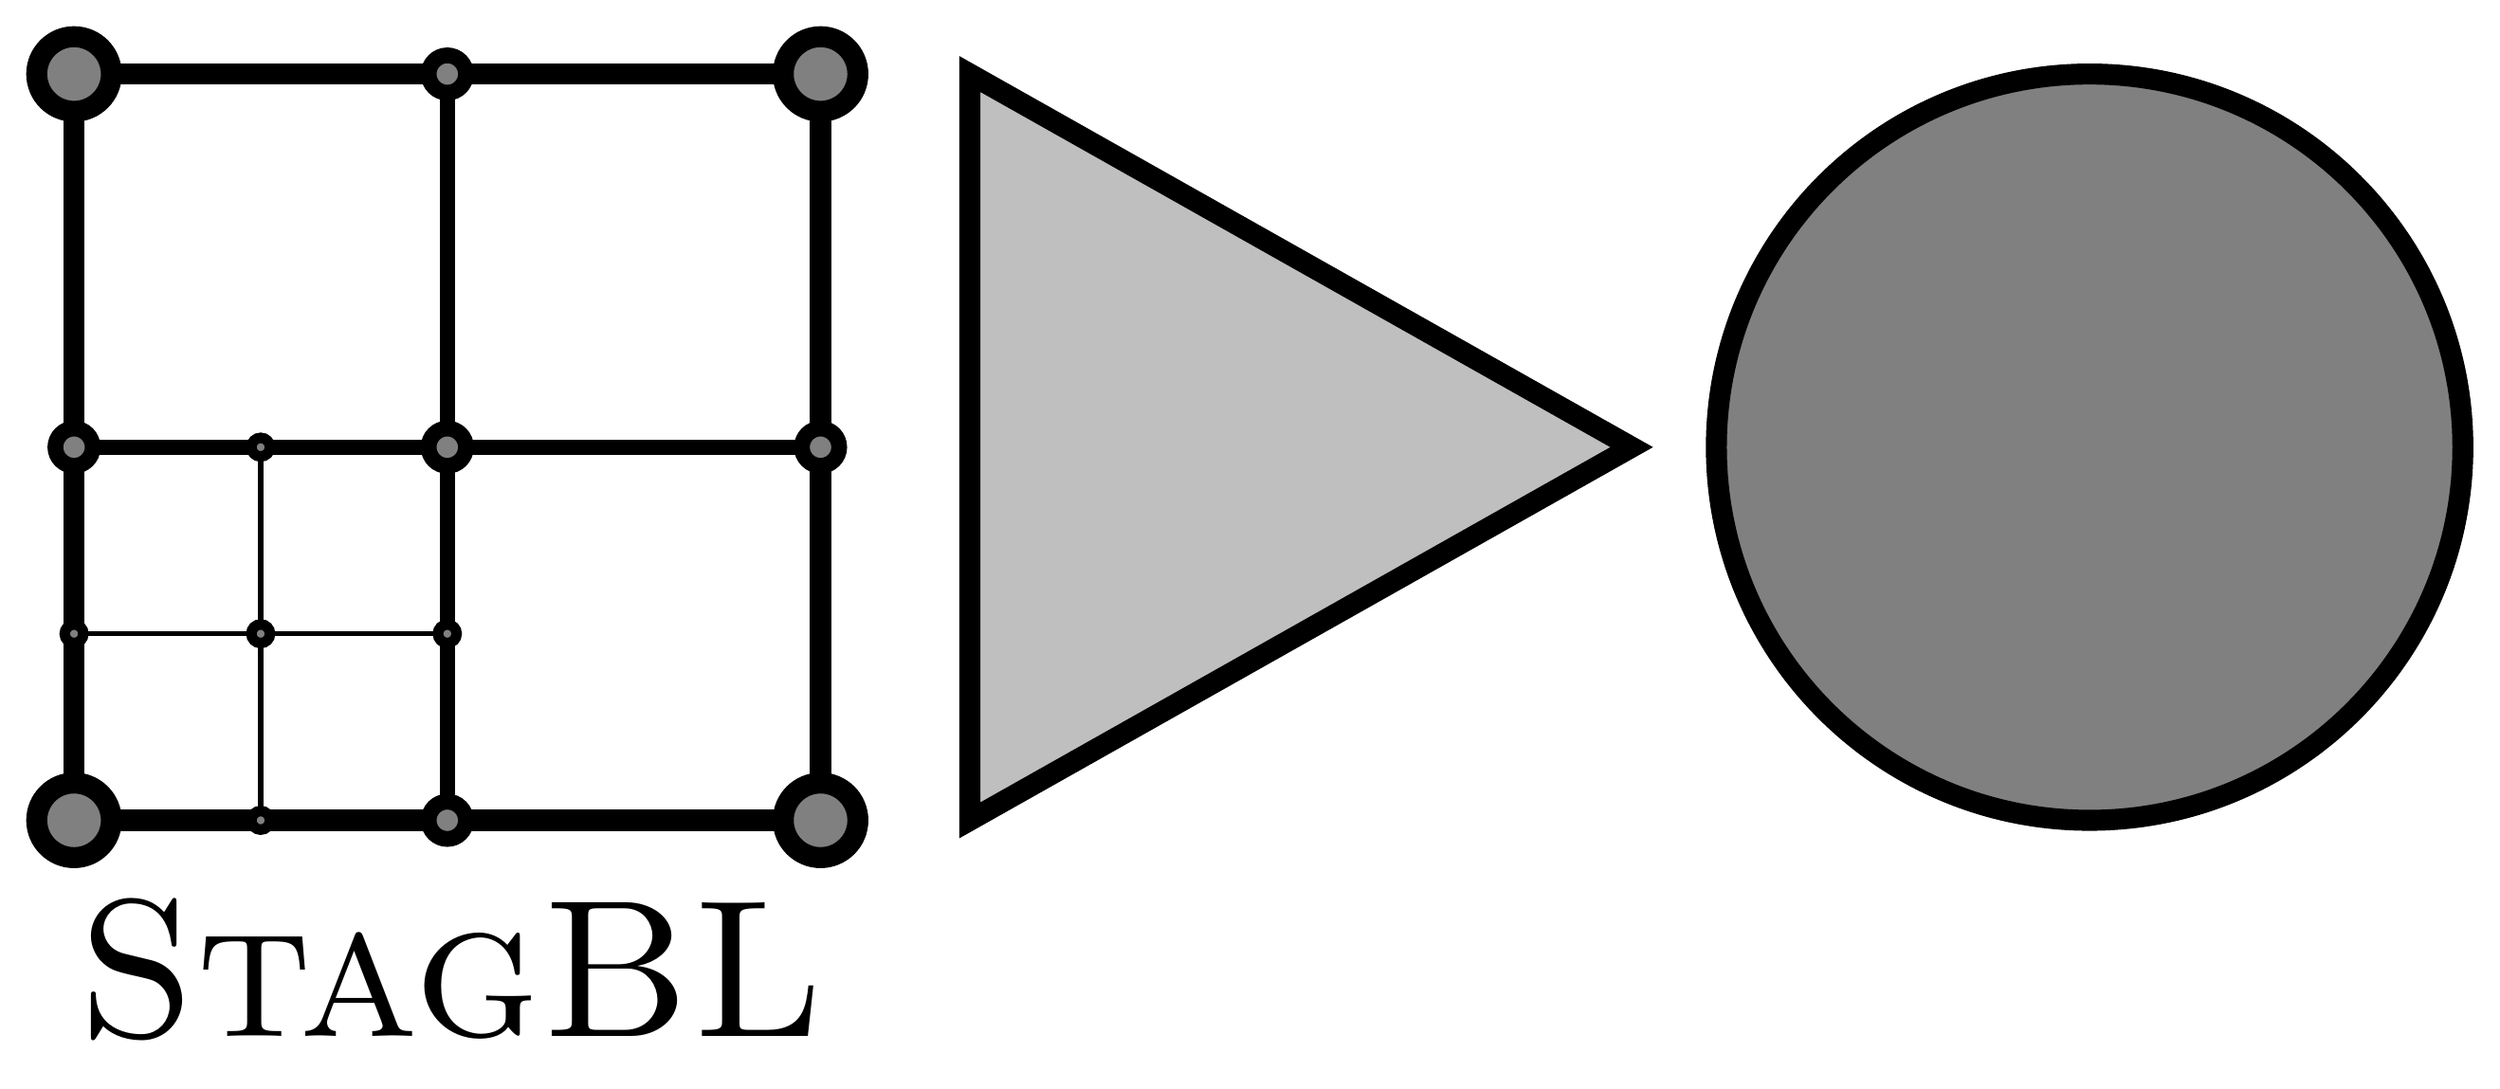
\begin{tikzpicture}
  [
  node1/.style={radius=0.5,draw=black,fill=black!50,line width=8},
  node2/.style={radius=0.25,draw=black,fill=black!50,line width=6},
  node3/.style={radius=0.125,draw=black,fill=black!50,line width=4},
  ]

  % Grid
  \draw[line width=8] (0,0) -- (10,0) -- (10,10) -- (0,10) -- cycle;
  \draw[line width=6] (0,5) -- (10,5);
  \draw[line width=6] (5,0) -- (5,10);
  \draw[line width=2] (2.5,0) -- (2.5,5);
  \draw[line width=2] (0,2.5) -- (5,2.5);

  % Grid Nodes
  %\node at (0,0) [node1]{};
  \draw[node1] (0,0)     circle;
  \draw[node1] (10,0)    circle;
  \draw[node1] (10,10)   circle;
  \draw[node1] (0,10)    circle;
  \draw[node2] (5,0)     circle;
  \draw[node2] (5,5)     circle;
  \draw[node2] (0,5)     circle;
  \draw[node2] (5,10)    circle;
  \draw[node2] (10,5)    circle;
  \draw[node3] (0,2.5)   circle;
  \draw[node3] (2.5,0)   circle;
  \draw[node3] (2.5,2.5) circle;
  \draw[node3] (5,2.5)   circle;
  \draw[node3] (2.5,5)   circle;

  % Triangle
  \draw[line width=8,fill=black!25] (12,0) -- (12,10) -- (20.866,5) -- cycle;

  % Circle
  \draw[line width=8,fill=black!50] (27,5) circle [radius=5];

  % Text
  \node[align=left,scale=3] at (5.05,-2) {\Huge\textsc{StagBL}};

\end{tikzpicture}
\end{document}
